\subsection{Main implementation}
After many tries and research we came up with a really simple method of dealing with the MPI problem. Our method needs in addition to the number of elements also a processor amount of a power of two. We used the iterative FFT method as base. Since the FFT splits the array into even and odd parts, we used this to our advantage. There are actually just two notable parts of the algorithm which are doing the "MPI-things":
\begin{lstlisting}
for(int k=rank;k < i/2;k+=size)
\end{lstlisting}
This is the second of the three \textit{for} loops in the iterative algorithm. This splits the loop into evenly sized work-parts. Each iteration never crosstalks, which is perfect for parallelism.\newline
The second important part:
\begin{lstlisting}
if(i <= size && rank < i)
	sprayData(i, len);
\end{lstlisting}
\begin{lstlisting}
if(rank +i/2 < i){
	MPI_Send(out, len, MPI_DOUBLE_COMPLEX,
			rank + i/2, rank,MPI_COMM_WORLD);
}else{
	MPI_Recv(out, len, MPI_DOUBLE_COMPLEX,
			 rank - i/2, rank-i/2, MPI_COMM_WORLD, &status);
}
\end{lstlisting}
This basicly sends information to the processor, which is supposed to calculated the odd part of rank's array. 
\subsection{additional implementation}

The algorithm we use lets some processors just wait till the lower rank processors are done. So we tried to avoid that and let all processors, which aren't working on the second ('k'-)loop, help each other in the inner ('j'-)loop. In theory this would let to the result of linear speedup, but sadly MPI\_Scatter and MPI\_Gather are super slow. We also only benchmarked method \textit{help2}. \textit{help} only uses MPI\_Send/Recv but does the equivalent. In early testing we just proved that 'advanced' MPI functions deliver better performance, as told in the lecture.

\subsection{Performance}

Since we need a cores amount of a power of two, we chose 32 jupiter hosts and evenly spread the cores. We didn't bother comparing e.g. 8 cores on one node and 1 core per 8 nodes, because we noticed some strong time differences in the early testphase. \newline
Here is a graph trying to show the relation between the time MPI\_Send and MPI\_Recv needs in relation to len/2 random iterations (max iterations of inner loop):
\begin{center}
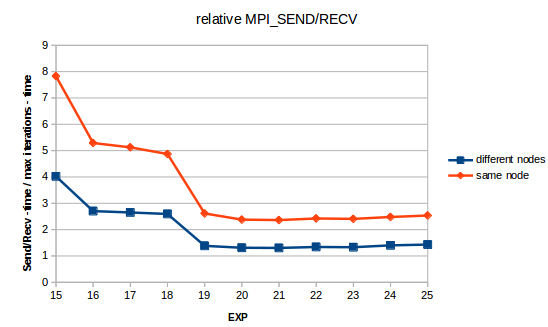
\includegraphics[width=\textwidth]{MPI_sr}
\end{center}
Communication between cores on the same node is obviously far slower. We do not know why there's this slope at 18-19. It always occurs and even on our speedup graphs you can see a hike around this area. 
\newline
Average speedup:
\begin{center}
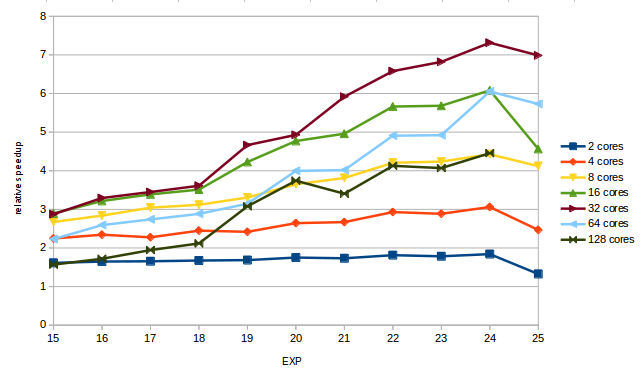
\includegraphics[width=\textwidth]{MPI_med}
\end{center}
Our best observed speedup:
\begin{center}
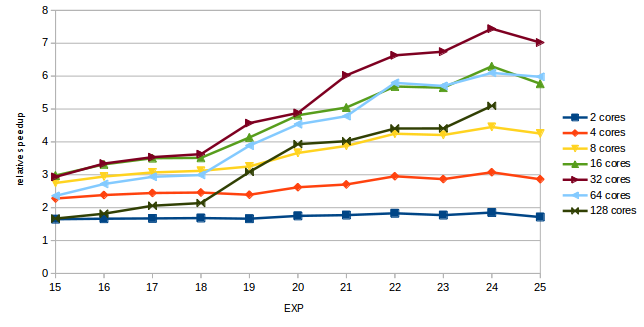
\includegraphics[width=\textwidth]{MPI_best}
\end{center}

Generally our MPI method loses a lot of time during the send and receive phase, especially at low exponents, where all iterations together are faster than the splits. As we kind of expected, most curves are rising in speedup. Similar to openMP and cilk but much smoother. This is most likely because of our simple split method which just works at the beginning and then lets all the cores do the rest without hard disturbance (fewer cores/node \(\implies\) fewer cache problems). \newline


We also include the best-case speedup-graph of our \textit{help2} method:
\begin{center}
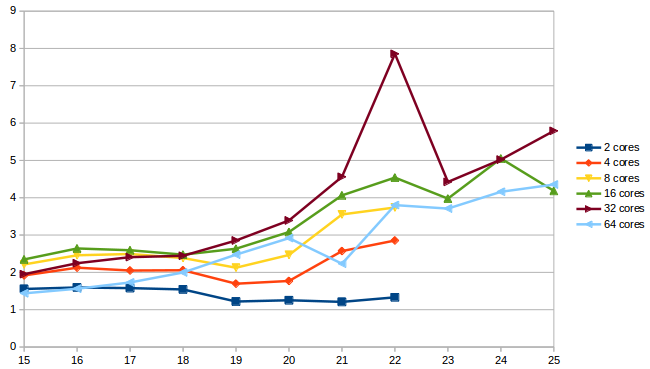
\includegraphics[width=\textwidth]{MPI_help2}
\end{center}

Out of hundred testcases there was one remarkable good one at \(2^{22}\) numbers. Even though MPI\_Scatter/Gather seem to be slow, which can be seen at the beginning of the graph in comparison to the other MPI graphs, it still catches up very nice at larger data amounts.
   
\subsection{Expectation}
We would expect an approximate linear speedup for large enough numbers. We tried to come up with a formula

There are \(2^{p}\) cores and array has length = \(2^{n}\)\newline
A ... average time needed for len/2 (=\(2^{n-1}\)) operations\newline
B... average time needed for MPI\_Send/Recv of \(2^{n}\) elements\newline\newline
\begin{math}
T(n, p) = A + \sum_{i=1}^{p} {A \over 2^i} + (n - p) {A \over 2^p} + p*B 
= A (1 + \sum_{i=1}^{p} {1 \over 2^i} + {n - p \over 2^p}) + p*B
\end{math}\newline
For big enough n and p:\newline
\begin{math}
T(n, p) \approx A (2 + {n - p \over 2^p})(+ p * B)
\end{math}\newline
This should be smaller than the sequential algorithm: \newline
\begin{math}
T(n, p) \approx A (2 + {n - p \over 2^p})+ p * B \leq T(n) = n * A
\implies {n - p \over 2^p} + {p*B \over A} \leq n - 2
\end{math}\newline
Assuming A and B are \(O(n)\):\newline
\begin{math}
\implies {n - p \over 2^p} + p \leq n - 2 
\implies {p*2^p + 2^{p+1} -p \over 2^p +1} \leq n
\implies O(p) \leq O(n)
\end{math}\newline
This is exactly our specification, so it is right for at least large n and p. That means according to our approximative formular \newline
\begin{math}
T(n, p) \approx A (2 + {n - p \over 2^p})
\end{math}\newline
We have not really created a linear speedup, but it is still nice enough.  